\documentclass{beamer}
\usepackage[russian]{babel}
\usepackage{amsmath,mathrsfs,mathtext}
\usepackage{graphicx, epsfig}
\usepackage[T1,T2A]{fontenc}
\usepackage[utf8]{inputenc}
\usetheme{Warsaw}%{Singapore}%{Warsaw}%{Warsaw}%{Darmstadt}
\usecolortheme{sidebartab}
\definecolor{beamer@blendedblue}{RGB}{15,120,80}

%----------------------------------------------------------------------------------------------------------
\title[\hbox to 56mm{Мультимоделирование, привилегированное обучение\hfill\insertframenumber\,/\,\inserttotalframenumber}]
{Использование мультимоделирования и привилегированного обучения для построения моделей оптимальной сложности. }
\author[]{\large Нечепуренко  Иван Олегович}
\institute{\large
Московский физико-технический институт \par Факультет Инноваций и Высоких Технологий \par Кафедра анализа данных}

\date{\footnotesize{2019 \par Москва}}

%----------------------------------------------------------------------------------------------------------
\begin{document}
%----------------------------------------------------------------------------------------------------------
\begin{frame}
%\thispagestyle{empty}
\titlepage
\end{frame}
%-----------------------------------------------------------------------------------------------------
\begin{frame}{Цели исследования}

\begin{block}{Цель работы}
Создать метод построения моделей
оптимальной сложности для задач обучения с учителем.  
\end{block}

\begin{block}{Проблема}
Во многих случаях устройства,  на которых решаются задачи машинного обучения, неспособны хранить и обрабатывать большие объемы данных, а также имеют слабую вычислительную мощность.
\end{block}

\begin{block}{Метод решения}
Во-первых, использовать априорную информацию, производимую более сложной моделью - учителем.
Во-вторых, научиться грамотно строить  композицию простых моделей
\end{block}

\end{frame}

%-----------------------------------------------------------------------------------------------------
\begin{frame}{Литература}
\textbf{Смесь моделей}

\begin{itemize}
  \item Yuksel Seniha Esen, Wilson Joseph N., Gader Paul D. Twenty Years of Mixture
of Experts // IEEE Transactions on Neural Networks and Learning Systems. 2012. 23, № 8. С. 1177–1193.
 - Большая обзорная статья
\end{itemize}

\textbf{Привилегированное обучение}

\begin{itemize}
  \item Learning using privileged information: Similarity control and knowledge
transfer. V.Vapnik, R.Izmailov. JMLR, 2015. - Использование привилегированного обучения
применительно к SVM.

    \item Unifying distillation and privileged information. B.Schlolkopf, V.Vapnik,
D.Lopez-Paz, L.Bottou. ICLR, 2016. - Обобщение подходов Вапника и Хинтона к
привилегированному обучению.

\end{itemize}

\end{frame}

%-----------------------------------------------------------------------------------------------------
\begin{frame}{Постановка задачи}
\begin{block}{Общая задача}
Набор объектов - $\mathbb{X}$.  У каждого объекта есть набор признаков,  лежащий в $\mathbb{R}^m$.  Такие значения можно задать матрицей 
$\mathbf{X} = [x_i]_{i = 1}^n$, где $x_i$ -  как раз вектор признаков $i$-го объекта. Также есть матрица ответов $\mathbf{Y} = [y_i]_{i = 1}^n$.  В общем случае задача - построить алгоритм $\hat{f}$, минимизирующий заданную целевую функцию $S(y_i, \hat{f}(x_i)) $
\end{block}

\begin{block}{Задача многоклассовой классификации.}
Когда $ y_i = [y_i^1, ..., y_i^r],$ при этом $ \forall k: 0 \leq y_i^k  \leq 1,$
$ \sum\limits_{i = 1}^r y_i = 1$, задача называется задачей классификации на $k$ классов. Функцией ошибки мы выберем  кросс-энтропию: 
$$S(y_i, \hat{f}(x_i)) =  - \sum\limits_{i=1}^r y_i^k \log \sigma(\hat{f}(x_i)^k), \sigma (\hat{y})^k = \frac{\exp y^k}{\sum\limits_{k' = 1}^{r} \exp y^{k'}} $$
\end{block}

\end{frame}

%-----------------------------------------------------------------------------------------------------
\begin{frame}{Постановка задачи}
\begin{block}{Задача декодирования}
Если матрица ответов состоит из действительных векторов  $y_i \in \mathbb{R}^r$, то задачам декодирования соответствуют следующие функции ошибки:
$$MAE(y_i, \hat{f}(x_i)) = || y_i - \hat{f}(x_i) ||_1,$$
$$MSE(y_i, \hat{f}(x_i)) = || y_i - \hat{f}(x_i) ||_2,$$
$$MAPE(y_i, \hat{f}(x_i)) = ||\frac{ y_i - \hat{f}(x_i)}{y_i} ||_1,$$
\end{block}

\end{frame}

%-----------------------------------------------------------------------------------------------------
\begin{frame}{Постановка задачи}


\begin{block}{Шлюзовая функция}
Пусть имеются модели $f_1, ..., f_k$.   Для каждого объекта $x$ определяется правдоподобие $\pi_k(x) \rightarrow [0, 1]$ $i$ - й модели на нем. 
$$ \pi_k(x, V) = \varsigma(g(x, \omega), V) = \frac{exp v^T_k g(x, \omega)}{\sum\limits_{i = 1}^k exp v_k' g(x, \omega)}$$
Здесь  $V = [v_1, .., v_k, \omega]$, $\varsigma$ - softmax, $g(x, \omega)$ - преобразование над $x$.
\end{block}


\begin{block}{Смесь экспертов}
Получив $\pi_i$, можно построить модель, задаваемую формулой 
$$ f_me(x) = \sum\limits_{i =1}^{k} \pi_i(x, V) f_i(x)$$
\end{block}

\end{frame}

%-----------------------------------------------------------------------------------------------------
\begin{frame}{Цели эксперимента}

    Рассмотрим задачу аппроксимации кусочно - гладкой функции   при помощи нескольких линейных. Для начала рассмотрим случай, когда "начальные" модели идеально описывают тот или иной участок  
\begin{figure}[!htb]
        \center{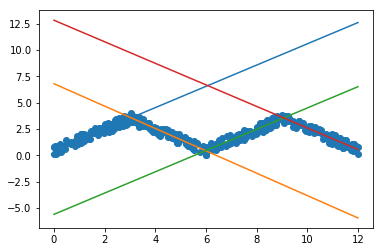
\includegraphics[width=10cm, height=5cm]
        {img/initial_task.png}}
      \end{figure}

\end{frame}

%-----------------------------------------------------------------------------------------------------
\begin{frame}{Тривиальные модели}
Классические нейронные сети приближают функцию только при достаточно большом кол-ве нейронов  в слое - порядка 500.
\begin{figure}[!htb]
       \center{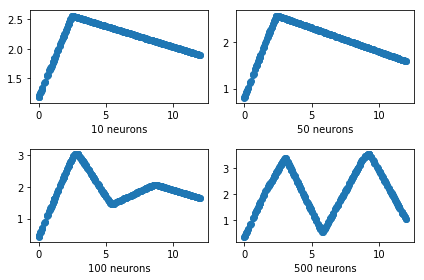
\includegraphics[width=\textwidth]
        {img/bare_tf.png}}
      \end{figure}

\end{frame}



%-----------------------------------------------------------------------------------------------------
\begin{frame}{Использование смеси экспертов}
\begin{block}{Способность мультимодели к фильтрации}
В качестве $\pi(x, V)$ Была использована нейросеть с $50$ нейронами для достижения примерно того же качества, как у  простой нейросети  с $50$ - ю электронами. Также выяснилось, что смесь экспертов выявляет незначимые модели $f_weak$ ($\pi_{weak} (x, V)$), и при удалении этих моделей качество оценки повышается. 
\end{block}


\begin{block}{Зависимость от изначальной иницилизации моделей}
Если в том же эксперименте  параметры "простых" моделей  подбирать случайно, только в около $10 \% $ случаев метод вообще  сходится. Значит, требуется как-то использовать дополнительную информацию.
\end{block}
\end{frame}


%-----------------------------------------------------------------------------------------------------
\begin{frame}{Использование привилегированной информации для смеси экспертов}
\begin{block}{Решение проблемы слабой сходимости}
Мы используем априорную информацию о принадлежности небольшого числа объектов конкретным экспертам, и именно на них 
обучаем простые модели. 

\begin{figure}[!htb]
       \center{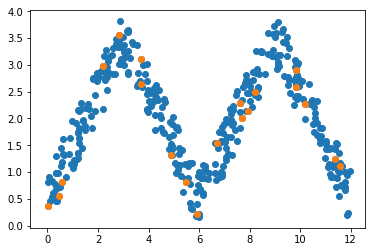
\includegraphics[width=10cm, height=3cm]
        {img/privileged_info.png}}
\end{figure}

\end{block}

\begin{block}{Результат}
В результате сходимость эксперимента увеличилась примерно до $70 \%$. 
\end{block}

\end{frame}

%-----------------------------------------------------------------------------------------------------
\begin{frame}{Фрейм}
\begin{block}{блок}
\end{block}
\end{frame}

%-----------------------------------------------------------------------------------------------------
\begin{frame}{Результаты эксперимента}
Была построена модель, которая довольно сильно снижает вычислительную сложность алгоритма. В нашем случае сложность алгоритма считается зависящей от числа нейронов в сети. При этом было привлечено минимальное количество привилегированной информации. 
\end{frame}


%-----------------------------------------------------------------------------------------------------
\begin{frame}{Заключение}
\begin{block}{Выводы:}
\begin{itemize}
  \item При достаточно хорошо подобранных начальных параметрах "исходных " моделей использование мультимоделирования помогает весьма сильно оптимизировать сложность модели при той же точности

  \item В случае же, когда исходные модели не очень хорошо настроены, метод может просто не сойтись.

\item При использовании некоторой "априорной"  информации, полученной отдельными "экспертами",  качество оценки и эффективность модели сильно увеличилась по сравнению с тем случаем, когда исходные модели иницилизировались протизвольно.

\end{itemize}
\end{block}
\end{frame}







\end{document} 